%!TeX root=../tese.tex
%("dica" para o editor de texto: este arquivo é parte de um documento maior)
% para saber mais: https://tex.stackexchange.com/q/78101

\chapter{Fundamentação teórica}

\section{Inteligência artificial}
% talvez por um sub cap de ml

Atualmente, a inteligência artificial (IA) permeia diversos 
momentos do cotidiano. Um exemplo é a empresa norte-americana 
de \textit{streaming} Netflix, que utiliza um conjunto de 
técnicas de inteligência artificial para recomendar conteúdo personalizado aos 
usuários da plataforma de acordo com os interesses 
particulares de cada um. Em particular para a Netflix, 
não há um modelo ou algoritmo único utilizado 
para todas as recomendações de conteúdo, essa tarefa é 
dividida em subtarefas realizadas por diferentes modelos de 
acordo com a atividade a ser realizada e os dados disponíveis. 
Por exemplo, a escolha de qual vídeo será exibido para 
o usuário ao logar no perfil da plataforma é executada por um 
modelo  diferente do que o que elenca os vídeos já assistidos que o 
membro pode continuar a ver.

Dessa forma, segundo \cite{netflix}, a empresa proporciona uma 
experiência única a cada indivíduo que acessa a plataforma. Essa 
estratégia tem o objetivo de aumentar a satisfação a longo prazo 
do cliente e garantir a retenção dos membros, uma vez 
que a plataforma é monetizada com assinaturas mensais. \cite{netflix}
ainda ressalta que a estratégia de utilizar inteligência 
artificial para as recomendações tem se refletido ao longo 
dos anos com uma melhora na taxa de retenção dos membros.

\begin{quote}
  \textit{"Therefore, the value of a recommender system can be measured by
the increase in member retention. Over years of the development of personalization and recommendation technologies, we have been able to repeatedly create meaningful
improvements in retention"} (\cite{netflix})
\end{quote}

Mas afinal, o que é inteligência artificial? O termo 
"inteligência artificial", de \textit{artificial intelligence} 
em inglês, foi elaborado por John McCarthy e utilizado 
oficialmente pela primeira vez em 1956 no seminário de 
Dartmouth, um \textit{workshop} sobre a área que reuniu os 
maiores estudiosos do ramo durante dois meses segundo \cite{aima}.
Entretanto, em 1950, Alan Turing já se perguntava se máquinas 
poderiam pensar e desenvolvia estudos e conceitos no tema que permanecem relevantes
como o Teste de Turing\footnote{Em \cite{turing}, Alan Turing propôs o 
Teste de Turing com a intenção de determinar se uma máquina era inteligente. O teste de Turing é uma variação 
do Jogo da Imitação em que um entrevistador deve fazer perguntas a dois jogadores, um 
humano e uma máquina, sem qualquer distinção. Ao final, o entrevistador deve
descobrir qual dos jogadores é uma máquina e qual é a pessoa. Se 
a máquina fosse capaz de enganar o entrevistador, seria considera
inteligente.}.
O termo "inteligência artificial, pode ser utilizado com
várias conotações, uma vez que não apresenta uma definição 
única e aceita, conforme 
relembra \cite{wang2019defining}. Uma possível definição,
segundo \cite{what-is-ai}, é a ciência e engenharia de 
construir máquinas inteligentes, em especial programas 
de computador, nesse contexto, inteligência é o aspecto
computacional da habilidade de atingir os objetivos.

\begin{quote}
  \textit{"The science and
  engineering of making intelligent machines, 
  especially intelligent computer programs. (...)
  Intelligence is the computational part of the ability 
  to achieve goals in the world."} John McCarthy
\end{quote}

Em 1959, o pioneiro em IA Arthur Samuel\footnote{Arthur Samuel
foi um engenheiro e um dos pioneiros em inteligência artificial,
desenvolveu um programa que jogava damas com humanos e aprendia
com cada jogada dos oponentes. O programa tornava suas jogadas mais 
assertivas ao calcular as probabilidades de cada jogada e é 
considerado uma das primeiras aplicações de aprendizado de máquina.
} descreveu 
aprendizado de máquina como o campo de estudo que dá aos 
computadores a habilidade de aprender sem serem específicamente
programados. Aprendizado de máquina ou \textit{machine learning} 
em inglês, portanto, compreende sistemas de inteligência 
artificial capazes de adquirir seu próprio conhecimento 
ao extrair padrões dos dados brutos de acordo com \cite{Goodfellow-et-al-2016}.
\textit{Machine learning}, então, configura-se como uma 
sub-área de inteligência artificial.


Já o aprendizado profundo, ou \textit{deep learning}, é uma 
categoria específica de algoritmos de \textit{machine learning}. 
De acordo com \cite{deeplearningbook}, caracteriza-se por 
modelos que fazem processamento de dados com neurônios 
matemáticos de forma a imitar o 
funcionamento do cérebro humano. Nesses algoritmos, a informação
é passada de camada em camada até obter a saída, trata-se, portanto,
de redes neurais com várias camadas ocultas de neurônios 
segundo \cite{d2l}. 

A relação entre inteligência artificial, aprendizado de 
máquina e aprendizado profundo pode ser vista na 
imagem \ref{fig:ia_ml}.
% repetindo algumas vezes a mesma coisa

\begin{figure}[H] 
  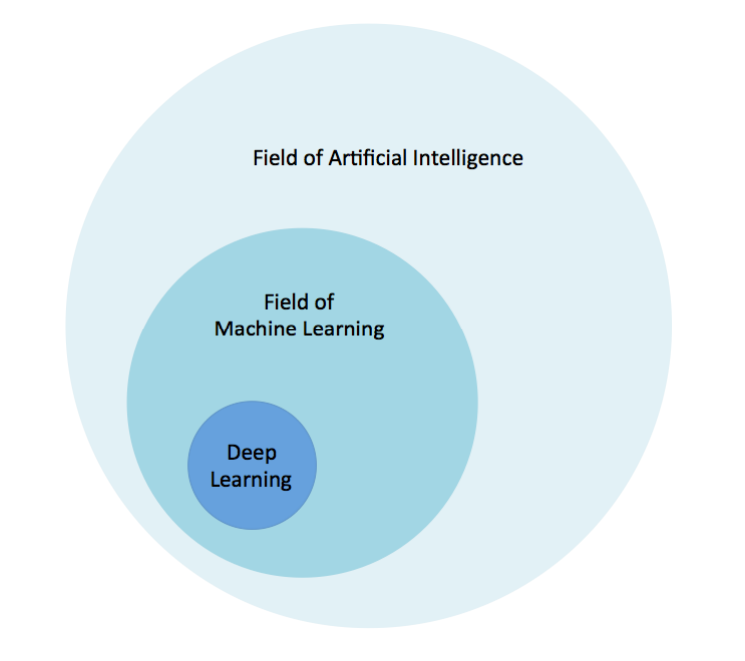
\includegraphics[width= 10cm]{../figuras/ia_ml.png}
  \caption{Relação entre inteligência artificial, aprendizado de máquina e aprendizado profundo (\cite{dl-oreilly})}
  \label{fig:ia_ml}
\end{figure}

\section{Tarefa}
 
Os modelos de \textit{machine learning} podem realizar várias categorias 
de tarefas, dentre elas a regressão e a classificação, a 
depender da atividade realizada pelo algoritmo.
Neste trabalho,  foram utilizados modelos de regressão onde o objetivo é prever um valor real a 
partir dos dados de entrada de acordo com \cite{Goodfellow-et-al-2016}.
É possível, então, descrever cada \textit{input} dos modelos como um vetor $x$ com 
$n$ atributos (\textit{features}) tal que
$x \in \mathbb{R}^n , x=\{x_1, x_2, ..., x_n\}$, neste trabalho, 
as \textit{features} utilizadas são indicadores econômicos, monetários,
sociais e da construção civil descritos na seção \ref{sec:dados}, já o 
processamento realizado pelos modelos de regressão pode ser descrito 
pela função $ f : \mathbb{R}^n \rightarrow \mathbb{R}$. 

Os modelos de classificação, por outro lado, têm como objetivo 
determinar a qual das $k$ categorias disponíveis um 
\textit{input} pertence de acordo com \cite{dl-oreilly}. Dessa forma, é utilizada uma função  
$ f : \mathbb{R}^n \rightarrow \{1,...,k\}$, quando 
$ f(x) = y$, o vetor de entrada $x$ foi classificado 
na categoria $y$. Um exemplo de tarefa de classificação,
seria determinar se uma operação com cartão de crédito 
é fraudulenta ou não, neste trabalho, contudo, não foi empregado 
tal tipo de modelo. 

Ainda segundo \cite{Goodfellow-et-al-2016}, os problemas de 
aprendizado de máquina também podem ser divididos entre
aprendizado não-supervisionado e supervisionado. No primeiro, 
o modelo recebe um conjunto de dados (\textit{dataset}) não 
rotulado e aprende propriedades da estrutura dos dados, 
um exemplo de aprendizado não supervisionado é a clusterização,
que consiste em dividir o conjunto de dados
em \textit{clusters} com amostras similares. No último, por sua vez, 
os dados de entrada estão associados a resultados conhecidos, 
chamados de \textit{labels} ou rótulos. Neste trabalho, utiliza-se aprendizado 
supervisionado para prever o consumo de cimento mensal nos 
estados da União a partir dos dados de entrada e compará-lo 
com o valor real 
do consumo e, assim, calcular a precisão do modelo.

\section{Modelos utilizados}

Neste trabalho, utilizou-se três categorias de modelos de aprendizado 
de máquina para prever a demanda por cimento: regressão linear, redes
neurais \textit{multi layer perceptron} e redes recorrentes. Foram testados, também,
três métodos de pré-processamento de dados (\textit{standard scaler, minmax 
scaler e power transformer}) e  diferentes arquiteturas de 
redes neurais ao alterar o número de camadas, a quantidade de neurônios
em cada camada, o tipo de camada, a função de ativação entre outras
configurações, com o objetivo de comparar 
o desempenho dos modelos e encontrar o que apresenta menor erro na previsão.

\subsection{Regressão linear}
\label{sec:reg_lin}

A regressão linear é um modelo de aprendizado de máquina que assume um relacionamento
linear entre a variável que será prevista (\textit{target}) e os dados de entrada.
Desse modo, seu objetivo é construir uma 
função que, para cada par\footnote{No
caso deste estudo, o par  $(x,y)$ é tal que 
$x$ representa o valor de cada
indicador descrito na seção \ref{sec:dados} em um estado e mês, já 
$y$ corresponde ao número de toneladas de cimento consumidas
por esse estado no mês e ano correspondente.} $(x,y)$, recebe como
entrada o vetor $x$ que corresponde às variáveis de \textit{input},
$x \in \mathbb{R}^k , x=\{x_1, x_2, ..., x_k\}$ e calcula coeficientes
$\beta = \{\beta_0, \beta_1, \dots, \beta_k\}$ para cada atributo de $x$,
além da constante $\beta_0$. O algoritmo, então, utiliza esses coeficientes para
prever um valor para a variável \textit{target}, $y$, sendo 
que $y \in \mathbb{R}$, segundo \cite{forecasting}. Seja,
então, $\hat{y}$ o valor previsto pelo modelo para um 
par $(x, y)$, a função que descreve a 
regressão linear, então é dada por

\begin{equation}
  \hat{y} = f(x) = \beta_0 + \beta_1 x_{1_i} + \beta_2 x_{2_i} + \dots + \beta_k x_{k_i} 
\end{equation}

É possível, logo, contruir uma matriz $X$ em que a linha $i$
corresponde ao vetor $x_i$ dos dados de entrada e 
cada coluna $j$ representa uma \textit{feature}. Pode-se, 
além disso, construir a matriz $\beta$ dos coeficientes associados 
a cada elemento da matriz $X$. Assim, o modelo
é dado por:

\begin{equation}
  \label{eq:reg_lin}
  y = X\beta + \epsilon
\end{equation}

Na equação \ref{eq:reg_lin}, $\epsilon$ é o vetor com o erro associado a cada umas 
das previsões, tal que $\epsilon_i = y_i - \hat{y_i} = y - (\beta_0 + \beta_1 x_1 + \beta_2 x_2 + \dots + \beta_k x_k )$.
Os coeficientes $\beta$ são calculados durante o treinamento 
do modelo utilizando o método do \textit{least squares estimation}
que visa minimizar a soma do erro quadrado associado às previsões, 
como descrito em:

\begin{equation}
  \sum_{i=1}^{n} \epsilon_i^2 = \sum_{i=1}^{n} (y_i - \hat{y_i}) = 
  \sum_{i=1}^{n} (y_i - (\beta_0 + \beta_1 x_{1_i} + \beta_2 x_{2_i} + \dots + \beta_k x_{k_i} ))
\end{equation}

Os coeficientes $\beta_1, \beta_2, \dots, \beta_k$ 
determinam como cada atributo de entrada afeta a previsão.
Por exemplo, se o coeficiente da variável $x_i$ for $\beta_i = 0$,
essa variável não tem influência no valor previsto pelo modelo. 
Caso o coeficiente seja positivo, por outro lado, um aumento 
no valor de $x_i$ resulta em aumento no valor previsto $\hat{y_i}$,
já se $\beta_i$ for negativo um aumento no valor de $x_i$ se reflete na 
diminuição no valor de $\hat{y_i}$. 


Na imagem \ref{fig:reg_lin}, há um exemplo de um modelo de regressão 
linear com apenas uma variável:

\begin{figure}[H] 
  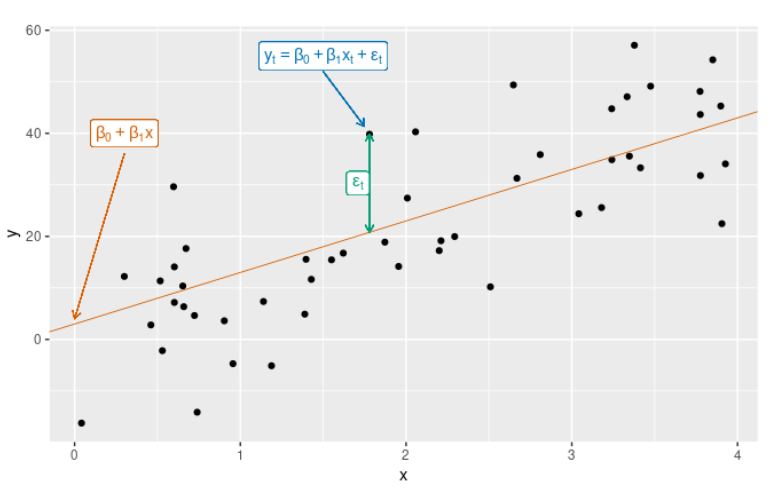
\includegraphics[width= 10cm]{../figuras/reg_lin.png}
  \caption{Exemplo de um modelo simples de regressão linear
  (\cite{forecasting})}
  \label{fig:reg_lin}
\end{figure}

Na  figura \ref{fig:reg_lin}, as observações $y_i$, estão 
representadas pelos pontos pretos, enquanto a linha em laranja
corresponde à previsão realizada pelo modelo. Observa-se que
o modelo não prevê com total exatidão os dados observados, há 
um erro associado a cada previsão, como o destacado em verde 
na ilustração, comportamento esperado já os fenômenos previstos são 
sujeitos a fatores externos e não lineares como os modelos matemáticos.


Por se tratar de um modelo mais simples, os resultados obtidos
com a regressão linear são utilizados neste trabalho como base 
para comparar o desempenho de modelos mais robustos.

\subsection{Redes neurais}

Redes neurais são modelos computacionais inspirados no funcionamento
do cérebro animal. O cérebro é formado por neurônios que se
conectam para transmitir informações sem a necessidade de 
uma unidade central de controle. Um neurônio biológico, então, 
é uma célula nervosa que se comunica com outros neurônios 
por meio de impulsos eletroquímicos. Essa comunicação é 
denominada sinapse e ocorre apenas se o impulso 
for forte o bastante para ativar a liberação de
químicos na fenda sináptica, de acordo com segundo \cite{deeplearningbook}. 
Um neurônio é composto de vários dendritos, 
um axônio e um corpo celular, como ilustrado em \ref{fig:neuron}. 

\begin{figure}[H] 
  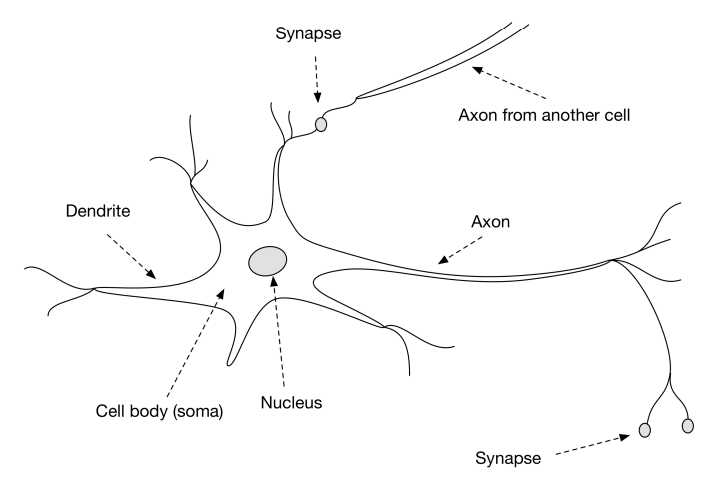
\includegraphics[width= 12cm]{../figuras/neuron.png}
  \caption{Ilustração de um neurônio biológico (\cite{dl-oreilly})}
  \label{fig:neuron}
\end{figure}

Destaca-se na figura \ref{fig:neuron}, informação chegando a um 
dendrito do neurônio em destaque
por meio de uma sinapse, além da comunicação com outra célula
por meio de outra sinapse iniciada no axônio 
do neurônio em questão. 

O processo de propagação da informação nos neurônios 
envolve as três partes da célula: dendritos, corpo celular
e axônio.
Os dendritos recebem informações de neurônios vizinhos 
na forma de impulsos elétricos e são responsáveis 
por conduzi-las até o corpo celular. 
Ao chegar no local, a informação é processada e novos 
impulsos são gerados e repassados a outro neurônio 
através do axônio no processo de sinapse, segundo \cite{fund_deep_learning}
A estrutura e funcionamento dos neurônios biológicos inspiraram
os cientistas ao projetarem neurônios artificiais, como 
os \textit{perceptrons}. 

\subsubsection{Neurônios artificiais}

O \textit{perceptron}, foi desenvolvido em 1957 por Frank 
Rosenblatt, inspirado nos trabalhos de Warren McCulloch e Walter Pitts
\footnote{Em 1943, Warren McCulloch e Walter Pitts, em \cite{neuronio}, apresentaram a 
primeira ideia de neurônio artificial.}.
Trata-se de um modelo linear de classificação que 
recebe $n$ entradas e produz uma saída binária, como mostrado 
na ilustração simplificada \ref{fig:perceptron-simples},
conforme \cite{deeplearningbook}.
Esse modelo inicial apresentava limitações e foi evoluído com o passar do 
tempo, contudo, as redes neurais atualmente utilizam, em geral,
outro modelo de neurônio como ilustrado em \ref{fig:perceptron}.


\begin{figure}[H] 
  \centering
  \begin{subfigure}{7cm}
    \centering 
    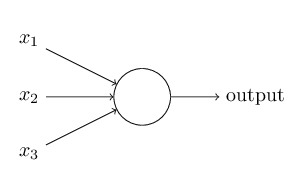
\includegraphics[width=7cm]{../figuras/perceptron-simples.png}
    \caption{Visão simplificada de um neurônio (\cite{deeplearningbook})}
    \label{fig:perceptron-simples}
  \end{subfigure}
  \hfill
  \begin{subfigure}{7cm}
    \centering
    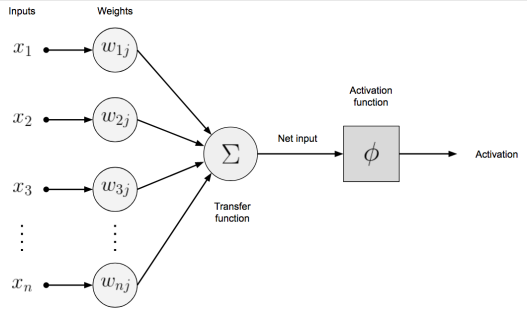
\includegraphics[width=7cm]{../figuras/perceptron.png}
    \caption{Ilustração da arquitetura de um 
    neurônio artificial (\cite{dl-oreilly})}
    \label{fig:perceptron}
  \end{subfigure}
\end{figure}

A figura \ref{fig:perceptron} mostra o funcionamento de 
um neurônio artificial. O neurônio apresenta $n$ entradas 
$x_i$, cada uma associada a um peso $w_i$, que expressa 
a importância das respectivas entradas para o valor de saída\footnote{ 
O peso atribuído a uma das entradas expressa a influência
dessa no \textit{output} do nó, de modo similar aos coeficientes calculados 
para cada atributo da regressão linear, explicada na seção \ref{sec:reg_lin}}.
O produto escalar entre os pesos e as respectivas entradas, 
chamada de \textit{net input}
na imagem \ref{fig:perceptron}, passa por uma função de 
ativação\footnote{Um detalhamento sobre as funções de 
ativação pode ser encontrado na seção \ref{sec:funcao_ativacao}} 
$\phi$ que determina a saída do neurônio. 
Além disso, um valor de \textit{bias} ou polarização é
adicionado ao produto escalar e possibilita que 
um neurônio que possua todas as entradas nulas
apresente saída não nula, dessa forma,
aumenta a capacidade de aproximação da rede. 
\cite{deeplearningbook}

É possível, então, traçar um paralelo entre o neurônio
artificial e o biológio. Em primeiro lugar, as entradas 
$x_i$ do neurônio  têm um funcionamento similar aos 
dentritos responsáveis 
por receber as informações que chegam à celula. Em segundo lugar,
o processamento matemático entre as entradas e os pesos 
tem comportamento similar ao corpo 
celular do neurônio biológico, que processa a informação 
recebida. Por fim, a função de ativação é responsável por modelar o 
\textit{output} que será repassado às camadas seguintes como uma das entradas
assim como o neurônio repassa, por meio de sinapses, os impulsos processados
a outros neurônios.


Seja $x$ o vetor das $n$ entradas do neurônio, então
$x \in \mathbb{R}^n, x=\{x_1, x_2, ..., x_n\}$ e seja 
$w$ o vetor com os pesos associados a cada entrada, 
$w \in \mathbb{R}^n, w=\{w_1, w_2, ..., w_n\}$. Além disso,
seja $b$ o valor de \textit{bias} e $\Phi$ a função de ativação.
Dessa forma, o \textit{output} de um neurônio é dado por:
 
\begin{equation}
  h_{w,b} = \Phi(w \cdot x + b)
\end{equation}

Essa saída é utilizada como uma das entradas dos neurônios
na camada seguinte, de modo a formar a estrutura das redes 
neurais. 


Os neurônios,
então, formam a unidade que compõe as redes neurais artificiais,
como ilustrado na figura \ref{fig:redeneural}:

\begin{figure}[H] 
  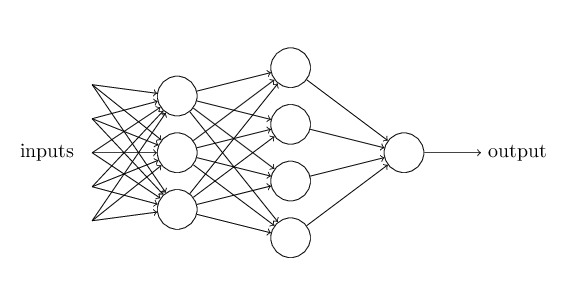
\includegraphics[width= 12cm]{../figuras/rede-neural.png}
  \caption{Ilustração de uma rede neural simples.(\cite{deeplearningbook})}
  \label{fig:redeneural}
\end{figure}

A imagem \ref{fig:redeneural} representa uma simplificação de uma 
rede neural. Pode-se observar o fluxo da informação, primeiro recebida pelos 
neurônios de uma camada, então processada nessas unidadades e, por fim, repassada à camada 
seguinte, até obter a saída final da rede. Em particular, é representada uma
rede \textit{feed forward}, uma vez que não há conexões entre neurônios de uma 
mesma camada nem conexões entre uma camada e a anterior. A informação então 
se propaga apenas no sentido da camada de entrada em direção à final, de saída.
As camadas intermediárias são chamadas de camadas ocultas ou \textit{hidden layers}.


\subsubsection{Função de ativação}
\label{sec:funcao_ativacao}

A função de ativação determina se um neurônio será ativado, ou seja, 
se a saída propagada para a camada seguinte. Enquanto os pesos 
e o \textit{bias} realizam uma transformação linear nos dados 
de entrada, a função de ativação aplica uma transformação não
linear, assim, possibilita que a rede neural resolva
problemas não lineares e complexos, como reconhecer padrões de 
escrita, conforme \cite{deeplearningbook} e \cite{zhang2021dive}. 

A função de ativação é um atributo de cada uma das camadas 
da rede e é escolhida de acordo com a tarefa que será 
executada. Por exemplo, a função sigmóide é recomendada
 para problemas de classificação. Neste trabalho, 
foram utilizadas: \textit{rectified linear unit} (ReLU) e \textit{swish}.

\subsubsection{Rectified linear unit (ReLU)}

A função ReLU, do inglês \textit{rectified linear unit}, é a
função de ativação mais popular atualmente, uma vez que apresenta bom desempenho 
em diferentes tarefas, de acordo com \cite{dl-oreilly}. A função ReLu é dada por:

\begin{equation}
  f(x) = max(0,x)
\end{equation}

A derivada da função, utilizada nos modelos de \textit{machine learning}
para atualizar os pesos e \textit{bias} no treinamento da rede, é zero, quando 
a entrada é nula, ou uma constante, caso contrário. Dessa
forma, a ReLU não sofre do problema da dissipação do gradiente\footnote{Um 
detalhamento sobre o problema da dissipação do gradiente está na seção \ref{sec:vanishing_gradient_problem}.} como
outras funções de ativação. O gráfica da ReLU está ilustrado em \ref{fig:relu}.

\begin{figure}[H] 
  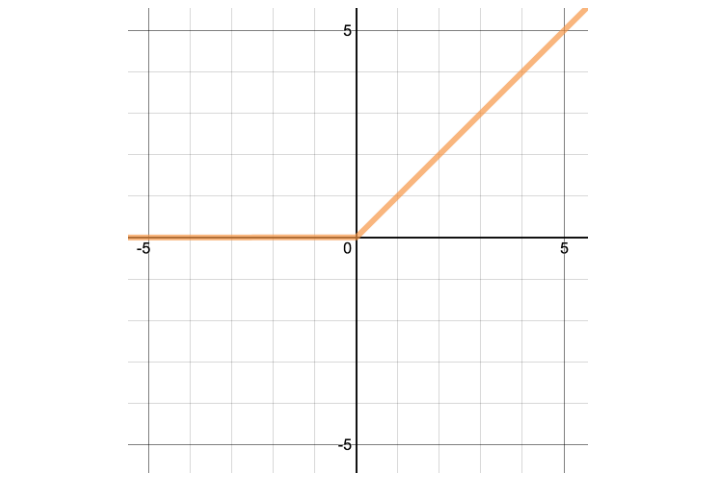
\includegraphics[width= 8cm]{../figuras/relu.png}
  \caption{Rectified linear unit (ReLU) (\cite{dl-oreilly})}
  \label{fig:relu}
\end{figure}

\subsubsection{Swish}

A função \textit{swish} foi proposta por pesquisadores da 
Google em \cite{swish}, com a promessa de apresentar desempenho igual 
ou superior à ReLU em redes neurais profundas. A \textit{swish} é uma função 
não monótona\footnote{Uma função definida como $f: I \rightarrow \mathbb{R}$
é monótona se é não crescente no intervalo $I$ ou não decrescente em $I$.} e 
suave\footnote{Uma função $f$ é suave se possui derivada de todas as ordens.},
cuja fórmula é dada por:

\begin{equation}
  f(x) = x \cdot sigmoid(x) = \frac{x}{1+e^{-x}}
\end{equation}


O gráfico da função é similar ao da ReLU e pode ser observado em \ref{fig:swish}.

\begin{figure}[H] 
  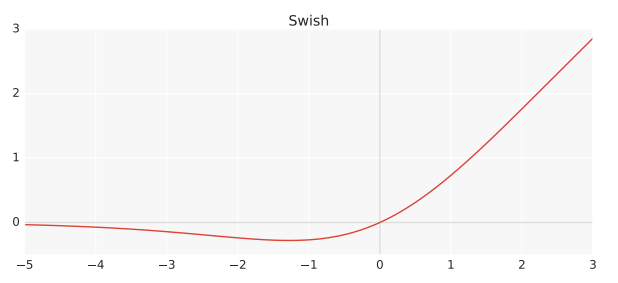
\includegraphics[width= 12cm]{../figuras/swish.png}
  \caption{Função \textit{swish} (\cite{swish})}
  \label{fig:swish}
\end{figure}


\subsubsection{Problema da Dissipação do Gradiente}
\label{sec:vanishing_gradient_problem}

De acordo com \cite{neuralnetworksanddeeplearning} aprendizado de uma rede neural ocorre ao alterar os valores dos pesos
e \textit{bias} dos neurônios de acordo com a função de custo, também conhecida 
como \textit{loss function}. Sejam $x$, $w$ e $b$ os conjuntos de entradas,
pesos e \textit{bias} da rede, respectivamente, a função de custo, então, é dada por:

\begin{equation}
  C(w,b) = \frac{1}{2n}\sum_x || y(x) - a ||^2
\label{eq:func_custo}
\end{equation}

Na equação da função de custo \ref{eq:func_custo}, $y(x)$ representa o vetor com as resposta
que a rede tenta prever, $a$ representa o vetor de \textit{output} da rede e 
$n$ é o número total de entradas de treino. É possível, então, calcular o gradiente
associado ao $j$-ésimo neurônio da $i$-ésima camada:

\begin{equation}
  \delta_j^i = \frac{\partial C}{\partial b_j^i}
\label{eq:func_grad}
\end{equation}

Os gradientes dos neurônios de uma camada determinam quão rápido essa camada
aprende. Então, como $\delta^i$ é o vetor cujos elementos determinam a variação
dos pesos e \textit{bias} da camada $i$, ou seja, determinam 
o aprendizado da camada. 

O problema da dissipação do gradiente\footnote{O problema da dissipação do gradiente 
é conhecido em inglês como \textit{The vanishing gradient problem}.
} ocorre, então, quando os gradientes das camadas iniciais, durante o treinamento
da rede, ficam com valores muito próximos a zero, por isso, o aprendizado das 
camadas iniciais torna-se lento e custoso.

\subsection{Redes neurais \textit{multi-layer}}
  % dar uma melhorada -> parte do com o treinamento fornecido
  % se agredar -> combinação -> melhorar
  % redes de arquitetura multilayer ...
  % o "e feedforward" não tem nada a ver -> é um passo do treinamento  -> sequencia dos dados de entrada



  Redes neurais são modelos de \textit{machine learning} 
inspiradas no cérebro humano aonde o aprendizado ocorre 
ao se agregarem neurônios matemáticos que 
estabelecem conexões de acordo com o treinamento fornecido. 
Neste trabalho, aplicaram-se redes 
\textit{multilayer perceptrons} (MLPs), ou seja, que 
apresentam múltiplas camadas de neurônios 
e \textit{feedfoward}, onde a saída de 
uma camada de neurônios é utilizada como entrada para a camada seguinte, sem utilizar retropropagação.
          
        
\subsection{Redes Neurais Recorrentes}
\label{rnn}

Se por um lado as redes neurais tradicionais são projetadas
para realizar previsões sem modelar dimensão temporal, as redes
neurais recorrentes se diferem por capturar informação de contexto, ou seja,
histórico, para realizar previsões. Essa dimensão temporal, então, se dá por 
meio de ciclos nas conexões, ou \textit{feedback loops}, como mostrado na 
figura abaixo.


\begin{figure}[H]
  \centering
  \begin{subfigure}{7cm}
      \centering
      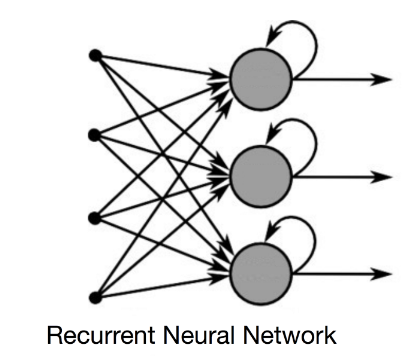
\includegraphics[width=7cm]{../figuras/redes/rnn.png}
      \caption{Redes neurais recorrentes}
  \end{subfigure}
  \hfill
  \begin{subfigure}{7cm}
      \centering
      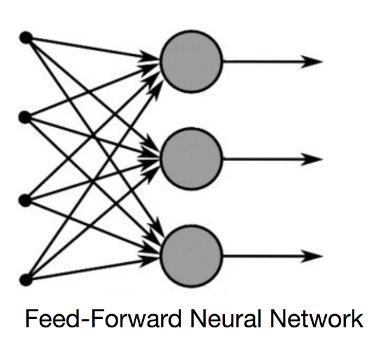
\includegraphics[width=7cm]{../figuras/redes/ff.png}
      \caption{Redes \textit{feed forward}}
  \end{subfigure}
\end{figure}

Dessa forma, os neurônios nas redes recorrentes recebem entradas de ativação 
de seu próprio estado atual e dos nós anteriores na rede, não apenas dos anteriores
na rede, como nas redes tradicionais.

As redes recorrentes, então, não recebem como entrada apenas um vetor de tamanho 
fixo como as redes \textit{feed forward}, seu \textit{input} é formado 
por vários vetores, um para cada \textit{time-step}. Na figura abaixo, o número
total de amostras corresponde ao campo "examples", o vetor com as 
variávies de entrada ao campo "inputs" ou "values per time step" (na 
figura de Recurrent Network Data) e o tamanho das sequências consideradas
pelo modelo ao "time steps". 

\begin{figure}[H] 
  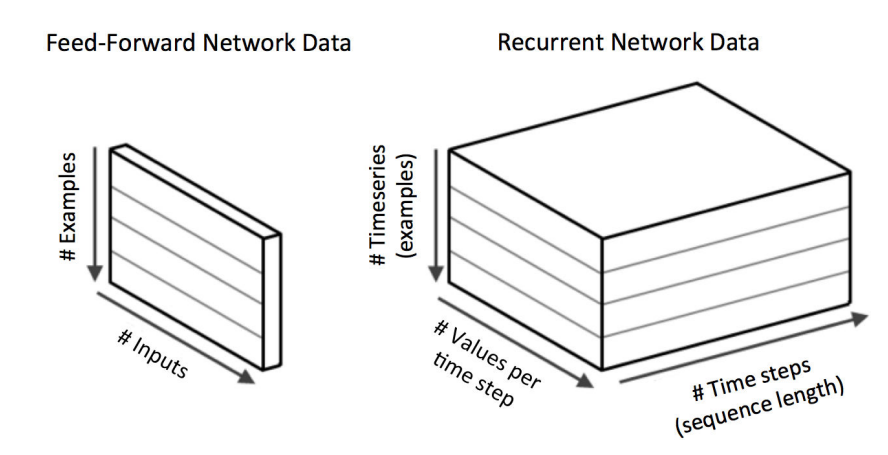
\includegraphics[width= 12cm]{../figuras/redes/input-rnn.png}
  \caption{Comparação entre a entrada de uma rede neural tradicional
  e um recorrente \cite{dl-oreilly}}
  \label{fig:input-rnn}
\end{figure}

Redes recorrentes são uma subclasse das redes neurais, contudo, possuem mais
de uma categoria, neste trabalho testaram-se as redes LSTM e GRU.

\subsubsection{LSTM}

As redes Long Short Term Memory (LSTM) foram introduzidas em 1997 por Hochreiter 
and Schmidhuber\footnote{\cite{lstm-origem}} e são a variação mais utilizada das redes
neurais recorrentes atualmente, por exemplo para classificar séries temporais, 
reconhecimento de fala e de escrita a mão. Redes LSTM apresentam células de 
memória conectadas, o conteúdo dessas células é modulado pelo \textit{input gate} e o \textit{forget gate},
por exemplo, se ambos estiverem fechados em um tempo o conteúdo da célula permanecerá 
o mesmo no tempo em questão e no próximo. Essa estrutura permite que a informação
seja retida ao longo do tempo e evita o problema do \textit{vanishing gradient} que 
ocorre com a maioria das redes recorrentes.

As redes neurais LSTM apresentam uma arquitetura diferente 
das redes tradicionais, uma vez que há ciclos de \textit{feedback}
nas conexões entre as células. Para melhor ilustrar essa 
arquitetura, \cite{dl-oreilly} utiliza a visualização \textit{flat} 
ou achatada das redes neurais, na qual as células de uma mesma 
camada da rede estão representadas como um único nó.
Pode-se observar essa representação em \label{fig:comparacao-ff-flat-normal},
na imagem \ref{fig:arq-ff} está a representação tradicional 
de uma rede neural \textit{feed forward}, já em em 
\ref{fig:arq-ff-flat} está a mesma rede com a represetnação 
achatada.

\begin{figure}[H]
  \centering
  \begin{subfigure}{7.5cm}
      \centering
      \label{fig:arq-ff}
      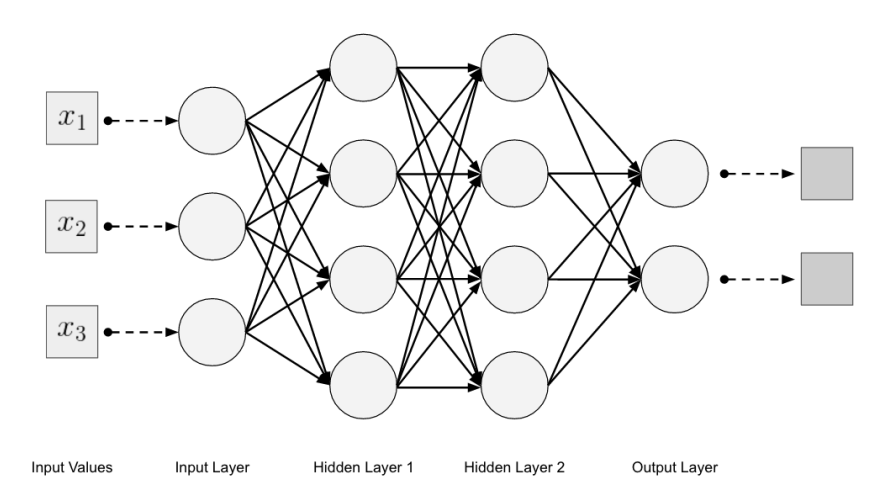
\includegraphics[width=7.5cm]{../figuras/redes/arq-ff.png}
      \caption{Arquitetura de rede neural \textit{feed forward}}
  \end{subfigure}
  \hfill
  \begin{subfigure}{7.5cm}
      \centering
      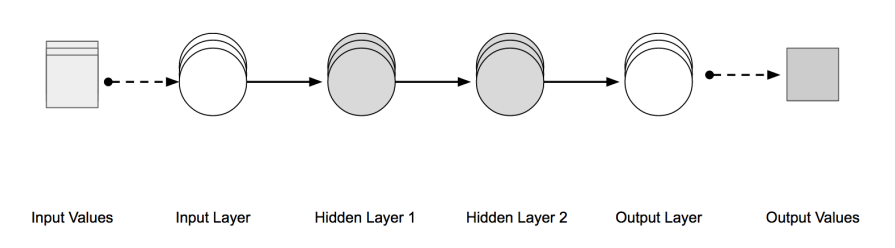
\includegraphics[width=7.5cm]{../figuras/redes/arq-ff-flat.png}
      \caption{Visão \textit{flat} (achatada) arquitetura de rede neural \textit{feed forward} }
      \label{fig:arq-ff-flat}
  \end{subfigure}
  \label{fig:comparacao-ff-flat-normal}
\end{figure}

As redes LSTM introduzem o conceito de conexão entre a saída de uma das 
camadas ocultas da rede neural com a entrada da mesma camada. A partir desse
ciclo, obtém-se entradas de tempos anteriores como parte da informação que 
chega à rede neural no tempo atual. Na figura \ref{fig:arq-rnn-flat}, essas 
conexões recorrentes são representadas como as setas que saem de uma célula e 
atingem a mesma célula, uma vez que utiliza-se a representação achatada.
A imagem \ref{fig:arq-rnnff}, por sua vez, representa a rede LSTM desenrolada 
atráves do eixo do tempo.

\begin{figure}[H]
  \centering
  \begin{subfigure}{7.5cm}
      \centering
      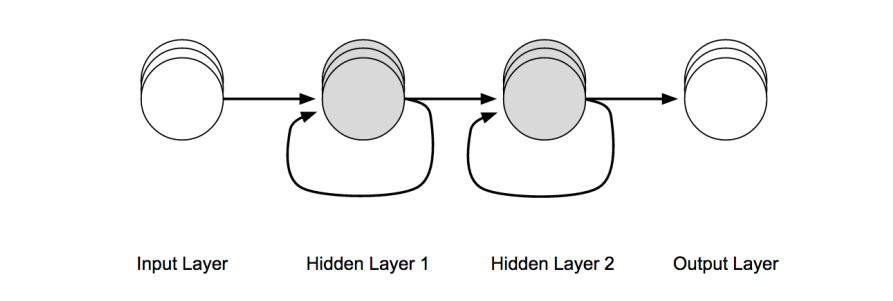
\includegraphics[width=7.5cm]{../figuras/redes/arq-rnn-flat.png}
      \caption{Visão \textit{flat} (achatada) arquitetura de rede neural LSTM }
      \label{fig:arq-rnn-flat}
  \end{subfigure}
  \begin{subfigure}{7.5cm}
    \centering
    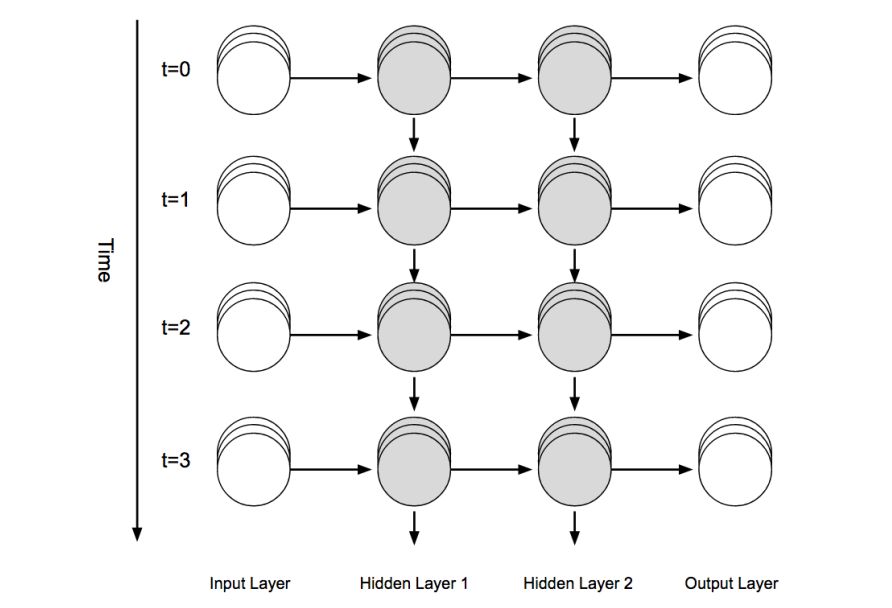
\includegraphics[width=7.5cm]{../figuras/redes/arq-rnn.png}
    \caption{Visão da rede neural LSTM ao longo do tempo}
    \label{fig:arq-rnnff}
  \end{subfigure}
  \hfill
  \label{fig:comparacao-rnn-flat-normal}
\end{figure}

As unidades que formam cada uma das camadas de uma LSTM são uma variação dos
neurônios artificiais clássicos. Essas unidades, representadas em \ref{fig:lstm-cell},
 permitem que a rede mantenha o estado
ao longo tempo e apresentam dois tipos de 
conexões: conexões vindas da camada anteriores e vindas \textit{outputs} dessa
mesma unidade em tempos anteriores.

\begin{figure}[H]
  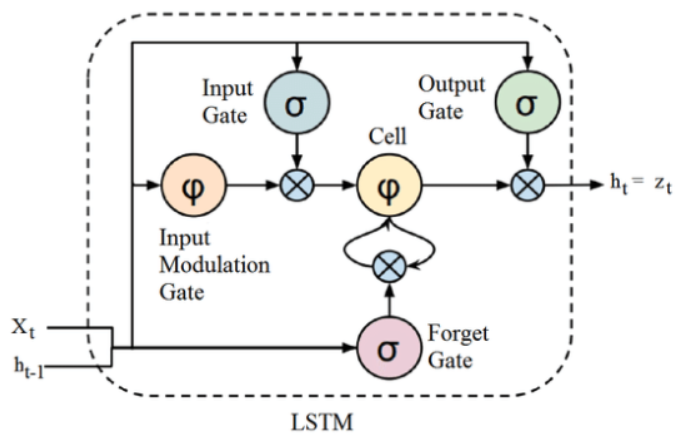
\includegraphics[width=9cm]{../figuras/redes/lstm-cell.png}
  \caption{Célula de memória de rede LSTM \cite{deeplearningbook}}
  \label{fig:lstm-cell}
\end{figure}

A unidade LSTM recebe duas entradas, a observação no tempo atual e a saída do 
último estado oculto. Nas unidades LSTM, a informação é retida nas células e as manipulações de memória 
são realizadas nos \textit{gates} (portões). O \textit{forget gate} é responsável
por remover informações que não são mais úteis para a célula, ou seja, pelo 
esquecimento, essa operação é realizada por meio de multiplicação de matrizes 
de pesos, adição de parâmetro de viés e função de ativação que fornece uma saída binária. 
O \textit{input gate}, por sua vez, adiciona informações úteis ao estado da célula
a partir da aplicação de funções sigmoides e tangente hiperbólica, além da multiplicação de vetores. 
Já o \textit{output gate} extrai informações úteis ao estado da célula atual 
para apresentar como saída da célula e entrada para a próxima com funções tangente
hiperbólica e sigmoide, além da multiplicação de vetores. \cite{deeplearningbook}

\subsubsection{GRU}

As GRU, sigla para \textit{gated recurrent units} no inglês,
são unidades recorrentes similares às LSTM. Enquanto as unidades
das redes LSTM apresentam dois estados passados entre as células, 
estado da célula e estado oculto, que carregam memória, respectivamente,
de longo e curto prazo, as unidades GRU apresentam apenas um 
estado oculto carregado ao longo do tempo e capaz de manter
as dependências de curto e longo prazo ao mesmo tempo. A 
estrutura das unidades GRU pode ser vista em \ref{fig:gru-cell}.

\begin{figure}[H]
  \centering
  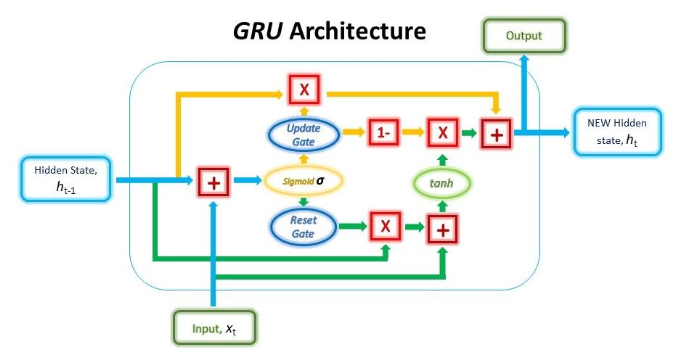
\includegraphics[width=9cm]{../figuras/redes/gru-cell.png}
  \caption{Unidade da rede GRU \cite{deeplearningbook}}
  \label{fig:gru-cell}
\end{figure}

As unidades GRU apresentam portões, assim como as unidades LSTM,
para controlar o fluxo de informações. O \textit{reset gate}, ou
portão de redefinição, é responsável por controlar quais informações 
das etapas anteriores serão mantidas com as da etapa atual por meio 
da função sigmoide e multiplicação de vetores. O \textit{update gate},
por sua vez, tem como objetivo determinal quanto das informações
armazenadas no estado oculto anterior devem ser retidas para 
o futuro.


\subsection{Normalização}
\label{sec:scaler}

O objetivo da normalização dos dados, é garantior que as variáveis de entrada 
estejam na mesma escala. Esse processo é necessário não apenas para realizar melhor comparação entre variáveis 
com diferentes unidades, mas também para o melhor funcionamentos dos algoritmos 
de aprendizado, uma vez que se as \textit{features} estiverem em escalas diferentes
os pesos podem ser atualizados mais rápidos que outros.

\subsubsection{\textit{Standard scaler}}

O \textit{standard scaler} garante que as variáveis de entrada estejam em uma 
escala com as propriedades de uma distribuição normal, ou seja, média ($\mu$)
igual a zero e variância ($\sigma$) igual a um. Dessa forma, a operação 
realizada para aplicar o processo em um entrada $x$ é

\begin{equation}
  z = \frac{x - \mu}{\sigma}
\end{equation}

\subsubsection{\textit{Min-Max scaler}}

O \textit{min-max scaler} transforma os dados de modo que a 
escala dos dados tenha um itnervalo definido, em geral, entre
0 e 1.

\begin{equation}
  X_{norm} = \frac{X - X_{min}}{X_{max} - X_{min}}
\end{equation}